\section{Theorie}
\label{sec:Theorie}


Ein Serienresonanzkreis ist in Abbildung \ref{fig:serienreson} dargestellt.
Er besteht aus einer äußeren Spannungsquelle $U(t)$ und in Serie 
geschaltetem ohmschen Widerstand $R$, Spule mit Induktivität $L$ und Kondensator 
mit Kapazität $C$ (\cite{noltingbro}).

\begin{figure}
	\centering
	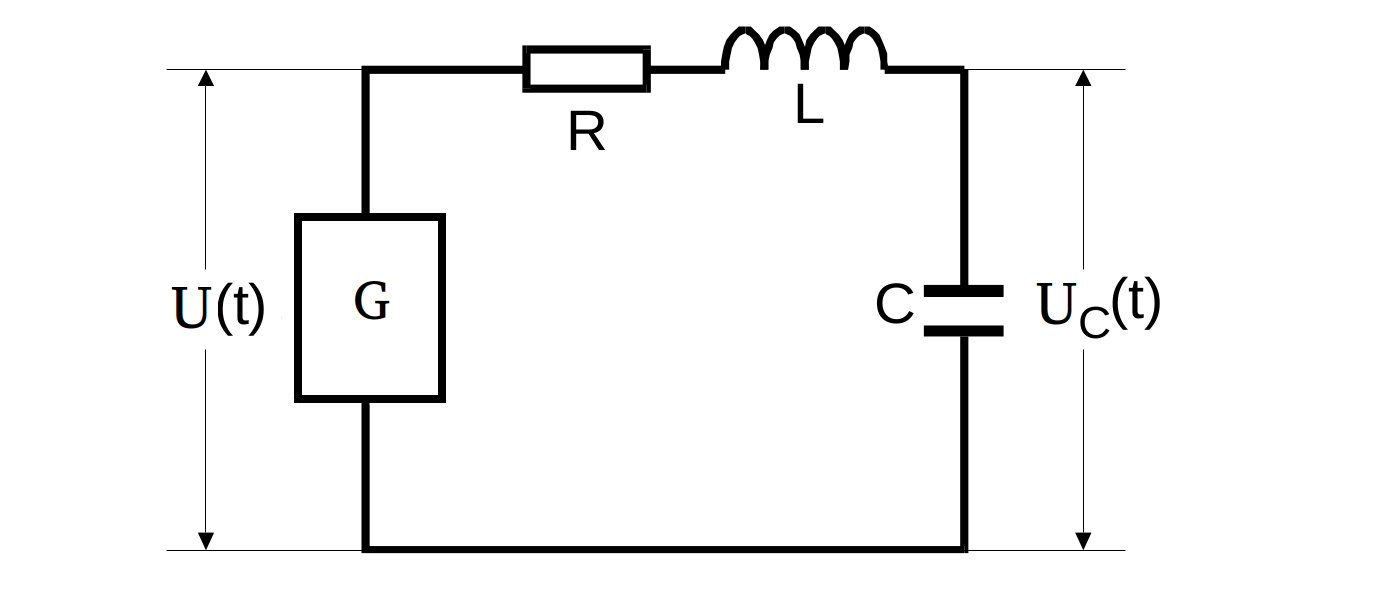
\includegraphics[width=0.7\textwidth]{Bilder/Aufbau.png}
	\caption{Schaltung eines Serienresonanzkreises \cite{Anleitung}}
	\label{fig:serienreson}
\end{figure}


\subsection{Ungedämpfte und gedämpfte Schwingungen}

Vorerst soll ein Serienresonanzkreis ohne äußere Spannungsquelle (Abbildung \ref{fig:serienresonlow}) -- also ein RLC-Kreis -- betrachtet werden.

Nimmt man an, dass zum Zeitpunkt $t=0$ ein bestimmter Energiebetrag im System vorhanden ist, 
werden elektrische Schwingungen erzeugt.
Diese lassen sich unterordnen in ungedämpfte und gedämpfte Schwingungen.

\textbf{Ungedämpfte Schwingungen} lassen sich in der Realität nicht erzeugen, da über ohmsche 
Widerstände elektrische Energie irreversibel in Wärmeenergie umgewandelt wird.
Sie entstehen also unter Vernachlässigung von ohmschen Widerständen.
Man betrachtet einen LC-Kreis, der mit einer Spule und einem Kondensator aus zwei 
Energiespeichern besteht. 
Dann alterniert die Energie verlustfrei als elektrische bzw. magnetische Feldenergie zwischen dem Kondensator und der Spule. 
Dies ist der Fall, da bei der Entladung des Kondensators ein Magnetfeld in der Spule erzeugt 
wird, welches daraufhin abgebaut wird und wiederum zur Aufladung des Kondensators mit 
umgekehrter Polung führt. Dieser Vorgang wird periodisch fortgesetzt, sodass die Energie zwischen Spule und Kondensator oszilliert.

\textbf{Gedämpfte Schwingungen} treten hingegen auf, wenn ohmsche Widerstände nicht vernachlässigt werden. 
Dann wird nämlich teilweise die vom Strom transportierte Energie irreversibel in Wärme 
umgewandelt und die Energie im RLC-Kreis ist so nicht erhalten. Im Folgenden sollen gedämpfte 
Schwingungen näher betrachtet werden.

Mit dem 2. Kirchhoffschen Gesetz erhält man aus dem Schaltkreis in Abbildung \ref{fig:serienresonlow} die Gleichung
\begin{equation*}
	U_{\text{R}}(t) + U_{\text{C}}(t) + U_{\text{L}}(t) = 0 \text{.}
\end{equation*}
Weiterhin erhält man mit dem Ohmschen Gesetz, dem Induktionsgesetz, der Spannung $U_{\text{C}} = \frac{Q(t)}{C}$ am Kondensator und dem Zusammenhang $I = \dot{Q}$ die Differentialgleichung
\begin{equation}
	\ddot{I} + \frac{R}{L} \, \dot{I} + \frac{1}{LC} \, I = 0 \text{,}
	\label{eqn:idgl}
\end{equation}
also eine lineare, homogene Differentialgleichung 2. Ordnung.
Diese lässt sich mit dem Ansatz 
\begin{equation}
	I(t) = I_0 \, \mathrm{e}^{i \omega t}
\end{equation}
lösen, wobei $I_0, \omega \in \mathbb{C}$.
Für $\omega$ ergibt sich
\begin{equation}
	\omega_{1,2} = i \, \frac{R}{2L} \pm \sqrt{\frac{1}{LC} - \frac{R^2}{4L^2}} \text{.}
\end{equation}
Mit den Definitionen
\begin{align}
	2 \pi \mu &:= \frac{R}{2L} & 2 \pi \nu &:= \sqrt{\frac{1}{LC} - \frac{R^2}{4L^2}}
	\label{eqn:defis}
\end{align}
lässt sich die allgemeine Lösung von Gleichung \eqref{eqn:idgl} schreiben als
\begin{equation}
	I(t) = \mathrm{e}^{-2 \pi \mu t} (I_1 \mathrm{e}^{i 2 \pi \nu t} + I_2 \mathrm{e}^{-i 2 \pi \nu t}) \text{,}
\end{equation}
wobei $I_1, I_2, \nu \in \mathbb{C}$.

Nun lassen sich die drei signifikanten Fälle für $\nu$ unterscheiden in denen $\nu$ entweder reell, komplex mit $\Im \nu \neq 0$ oder verschwindet.

\subsubsection{Der Schwingfall}
Damit $\nu$ reell ist, muss der Term in der Wurzel in der zweiten Gleichung \eqref{eqn:defis} 
positiv sein, also $\frac{1}{LC} > \frac{R^2}{4L^2}$ gelten.
Ist dies der Fall, erhält man als reelle Lösungsfunktion
\begin{equation}
	I(t) = I_0 \mathrm{e}^{-2 \pi \mu t} \cos(2\pi \nu t + \eta) \text{.}
	\label{eqn:schwingi}
\end{equation}
Dieser Fall entspricht einer gedämpften Schwingung mit der Frequenz $\nu$ und der Dämpfung
bedingt durch die monoton fallende Exponentialfunktion und wird daher als Schwingfall bezeichnet.
Weiterhin strebt die Amplitude von $I(t)$ wegen der Beschränktheit vom Kosinus für $t \to \infty$ gegen Null.
Die gedämpfte Schwingung ist in Abbildung \ref{fig:???} dargestellt.

Für die Periodendauer $T$ erhält man
\begin{equation}
	T = \frac{1}{\nu} = \frac{2 \pi}{\frac{1}{LC} - \frac{R^2}{4L^2}} \text{.}
\end{equation}
Betrachtet man nun den Fall $\frac{1}{LC} \gg \frac{R^2}{4L^2}$, gilt
\begin{equation}
	T \approx T_0 = \frac{2 \pi}{\omega_0} = 2 \pi \sqrt{LC} \text{,}
\end{equation}
die Thomsonsche Schwingungsformel. Die Periodendauer entspricht dann der Periodendauer der 
ungedämpften Schwingung.

Die Abnahmegeschwindigkeit der Amplitude ist durch $2 \pi \mu = \frac{R}{2L}$ festgelegt.
Man definiert die Abklingdauer $T_{\text{ex}}$ durch
\begin{equation}
	T_{\text{ex}} := \frac{1}{2 \pi \mu} = \frac{2L}{R} \text{.} 
\end{equation}

\subsubsection{Der Kriechfall}
Damit $\nu$ komplexwertig ist, muss $\frac{1}{LC} < \frac{R^2}{4L^2}$ gelten.
Ist dies der Fall, spricht man von dem Kriechfall oder auch der aperiodischen Dämpfung.
Dann gilt für $I(t)$ die Proportionalität
\begin{equation}
	I(t) \sim \exp(-(\frac{R}{2L} - \sqrt{\frac{R^2}{4L^2} - \frac{1}{LC}})t) \text{,}
\end{equation}
es liegt also kein Schwingungsvorgang vor, sondern es treten Relaxationsphänomene auf.

\subsubsection{Der aperiodische Grenzfall}
Der aperiodische Grenzfall tritt auf, wenn $\nu$ verschwindet, also wenn
\begin{equation}
	\frac{1}{LC} = \frac{R_{\text{ap}}^2}{4L^2}
\end{equation}
gilt.
Dann erhält man 
\begin{equation}
	I(t) = I_0 \mathrm{e}^{-\frac{R}{2L} t} = I_0 \mathrm{e}^{-\frac{1}{\sqrt{LC}} t} \text{.}
\end{equation}
Dieser Fall entspricht dem Fall mit der stärksten Dämpfung, die Amplitude nimmt monoton ab und 
konvergiert gegen Null.


\subsection{Erzwungene Schwingungen}

\textbf{Erzwungene Schwingungen} können mit einem Serienresonanzkreis realisiert werden (siehe 
Abbildung \ref{fig:serienreson}).
Dafür gibt der Spannungsgenerator eine Wechselspannung $U(t) = U_0 \mathrm{e}^{i \omega t}$ 
ab, mit der sich analog zu Gleichung \eqref{eqn:idgl} die Differentialgleichung
\begin{equation}
	LC \, \ddot{U_{\text{C}}} + RC \, \dot{U_{\text{C}}} + U_{\text{C}} = U_0 \mathrm{e}^{i \omega t}
\end{equation}
ergibt, mit der Kondensatorspannung $U_{\text{C}} = \frac{Q(t)}{C}$.
Diese lineare, inhomogene Differentialgleichung 2. Ordnung lässt sich mit dem Ansatz 
$U_{\text{C}} = U_{\text{C},0} \, \mathrm{e}^{i \omega t}$ lösen, wobei 
$U_{\text{C},0} \in \mathbb{C}$.
Einsetzen des Ansatzes in die Differentialgleichung liefert
\begin{equation}
	U_{\text{C},0} = \frac{U_0}{1-LC \omega^2 + i\omega RC}
\end{equation}
und damit wegen $|U_{\text{C}}| = |U_{\text{C},0}|$ ($\omega \in \mathbb{R}$)
die frequenzabhängige Kondensatorspannung zu
\begin{equation}
	\label{eqn:Uvonw}
	U_{\text{C}}(\omega) = \frac{U_0}{\sqrt{(1-LC \omega^2)^2 + \omega^2 R^2 C^2}} \text{.}
\end{equation}
Weiterhin gilt für die Phase $\phi(\omega)$ zwischen Kondensator- und Erregerspannung 
mit $\tan(\phi(\omega)) = \frac{\Im U_{\text{C},0}}{\Re U_{\text{C},0}}$
\begin{equation}
	\phi(\omega) = \arctan(\frac{-\omega R C}{1 - L C \omega^2}) \text{.}
	\label{eqn:phivonw}
\end{equation}

Die Frequenzabhängigkeit von $U_{\text{C}}$ in Gleichung \eqref{eqn:Uvonw} wird als 
Resonanzkurve bezeichnet.
Die Kondensatorspannung $U_{\text{C}}$ konvergiert für $\omega \to 0$  gegen gegen die 
Erregeramplitude $U_0$ und für $\omega \to \infty$ gegen Null.
Des Weiteren hat $U_{\text{C}}$ ein Maximum, bei der Frequenz
\begin{equation}
	\omega_{\text{res}} = \sqrt{\frac{1}{LC} - \frac{R^2}{2L^2}} \text{,}
\end{equation}
der Resonanzfrequenz.

In dem Fall $\frac{R^2}{2L^2} \ll \frac{1}{LC}$ spricht man von schwacher Dämpfung und es gilt 
$\omega_{\text{res}} \approx \omega_0$. Damit folgt $U_{\text{C,max}} > U_0$ mit
\begin{equation}
	U_{\text{C,max}} = \frac{1}{\omega_0 RC} U_0 = \frac{1}{R} \sqrt{\frac{L}{C}} U_0 \text{.}
\end{equation}
Weiterhin heißt der Faktor $\frac{1}{\omega_0 RC}$ Güte $q$ oder auch Resonanzüberhöhung eines 
Schwingkreises.

Eine weitere wichtige Kenngröße eines Schwingkreises ist die Breite der Resonanzkurve.
Sie ist ein Maß für die Schärfe der Resonanz und ergibt sich aus der Differenz von 
$\omega_+$ und $\omega_-$, den beiden Frequenzen, bei denen die Kondensatorspannung $U_{\text{C}}$ den Wert $U_{\text{C}} = \frac{1}{\sqrt{2}} U_{\text{C,max}}$ annimmt.
Mit der Näherung $\frac{R^2}{L^2} \ll \omega_0^2$ ergibt sich für die Breite der Resonanzkurve 
\begin{equation}
	\omega_+ - \omega_- \approx \frac{R}{L} \text{,}
\end{equation}
also auch der Zusammenhang zwischen Güte $q$ und Breite der Resonanzkurve zu
\begin{equation}
	q = \frac{\omega_0}{\omega_+ - \omega_-} \text{.}
\end{equation}

Zur Phasenverschiebung zwischen Kondensator- und Erregerspannung lässt sich anmerken, 
dass sie gemäß Gleichung \eqref{eqn:phivonw} für $\omega \to 0$ gegen Null geht und für 
$\omega \to \infty$ gegen $\pi$ konvergiert. 
An der Stelle $w_0^2 = \frac{1}{LC}$ ist die Phasenverschiebung $\phi = -\frac{\pi}{2}$ und 
$\phi = \frac{\pi}{4}$ bei
\begin{equation}
	\omega_{1,2} = \pm \frac{R}{2L} + \sqrt{\frac{R^2}{4L^2} + \frac{1}{LC}} \text{.}
\end{equation}
Damit gilt $\omega_1 - \omega_2 = \frac{R}{L}$ und damit lässt sich bei schwacher Dämpfung 
der Zusammenhang
\begin{equation}
	\omega_1 - \omega_2 \approx \omega_+ - \omega_-
\end{equation}
erkennen.
